\documentclass[letterpaper,12pt]{report}
\usepackage{pstricks}
\usepackage{amsmath}
\usepackage{wrapfig}
\usepackage{graphicx}

\begin{document}


% Title
\title{Basic Indirect Adaptive Control of a Differential Drive Robot with LQG\\EL 7253 Project}
\author{Griswald Brooks}
\maketitle
 
\begin{abstract}
While LQG control of a linear system provides optimal control and estimation, it depends on having an accurate system model.
At times, the parameters of the model will not be known exactly or will change at runtime.
This paper describes a basic indirect adaptive LQG controller and presents simulation results.
\end{abstract}

\tableofcontents

\chapter{Introduction}

\section{Concept and Motivation} \label{sec:concept}
LQG provides optimal control and estimation of linear systems given a sufficiently accurate system model. Identifying the system
parameters is sometimes unwieldy, especially if the system cannot be taken offline or runtime variable.
Inaccurate parameter identification can lead to poor controller performance or system instability.
If the control system can estimate the uncertain parameters at runtime, it can work to alleviate these short-comings and
be applicable to more systems without the need for the technician to identify system parameters at every implementation.

One method of adaptation is called direct adaptation. This involves adapting the control gains in order to improve system performance.
Another method is indirect adaptation. In this method, system model parameters are estimated and used to recompute state estimates and control gains.
In this work, a basic indirect adaptation method is presented where the model parameters are modified as a function of state error.

\begin{equation} \label{eq:changeParam1}
k_{n+1} = f(k_n, e)
\end{equation}

Where $k_{n+1}$ is the updated uncertain parameter, $k_n$ is the current parameter estimate, and $e$ is the current error between 
the state estimate and the state measurement.

\section{System Dynamics}

The system considered in this project a differential drive robot modeled in the plane. The body and wheels of the robot are modeled as three solid disks,
where the center of rotation is coincident with the center of mass of the robot body.

\begin{figure}[h]
	\centering
	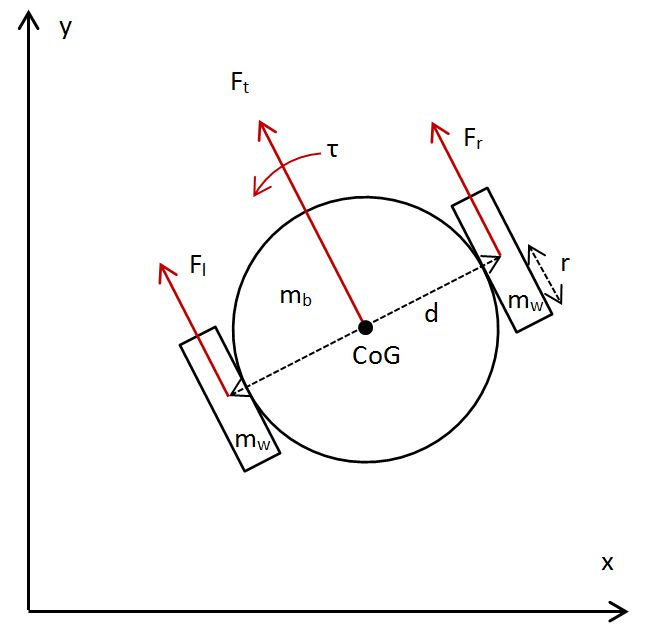
\includegraphics[width=0.5\textwidth]{Kinematics1.jpg}
	\caption{Differential Drive Diagram}
	\label{fig:ddDiagram1}
\end{figure}

In figure \ref{fig:ddDiagram1} $m_b$ and $m_w$ refer to the mass of the body and the mass of each wheel, respectively; $d$ and $r$ refer to the diameter of the
wheel base and the radius of each wheel; and $F_r$, $F_l$, $F_t$, and $\tau$ refer to the force exerted on the vehicle by the right and left wheels, the vehicle 
forward force and the vehicle torque about the center of gravity (CoG).

From \cite{ivanjko2010}, and taking the CoG and CoM to be coincident, the differential drive model is:

\begin{equation}
d_1\ddot\theta_r + d_2\ddot\theta_l = \tau_r - k_f\dot\theta_r
\end{equation}
\begin{equation}
d_2\ddot\theta_r + d_1\ddot\theta_l = \tau_l - k_f\dot\theta_l
\end{equation}
\begin{equation}
d_1 = \frac{m_br^2}{4} + \frac{I_br^2}{d^2} + I_w
\end{equation}
\begin{equation}
d_2 = \frac{m_br^2}{4} - \frac{I_br^2}{d^2}
\end{equation}

Where $\tau_x$ are the wheel motor input torques, $\ddot\theta_x$ and $\dot\theta_x$ are the wheel angular accelerations and angular velocities, $k_f$ is the viscous wheel friction, 
and $I_b$ and $I_w$ are the body and wheel inertias. This simulation took the inertia of the body and the wheels to be solid disks.

\begin{equation}
I_b = \frac{m_bd^2}{8}
\end{equation}
\begin{equation}
I_w = \frac{m_wr^2}{2}
\end{equation}

The dimensions utilized in the simulation were $m_b =$ 2.5 kg, $m_w =$ 0.05 kg, $d =$ 0.25 m, $r =$ 0.05m.

The wheel drive motors were modeled as first order systems.
\begin{equation}
\dot\tau = k_{bw}\tau + k_gu
\end{equation}
Where $k_{bw}$ is the motor bandwidth, $k_g$ is the input voltage gain, and $u$ is the input voltage.
Using a common hobby DC motor as a reference, $k_f$, $k_{bw}$, and $k_g$ were calculated as 0.0522, $20\pi$, and 0.5 respectively
to be reasonable estimates.

The full system model was taken as:
\begin{equation}
	\begin{bmatrix}
		\ddot\theta_r \\ \ddot\theta_l \\ \dot\tau_r \\ \dot\tau_l
	\end{bmatrix}
	=
	\begin{bmatrix}
		-k_fL^{-1} & L^{-1} \\
		0 & -K_{bw}
	\end{bmatrix}_{4x4}
	\begin{bmatrix}
		\dot\theta_r \\ \dot\theta_l \\ \tau_r \\ \tau_l
	\end{bmatrix}
	+
	\begin{bmatrix}
		0 \\ K_g
	\end{bmatrix}_{4x2}
	\begin{bmatrix}
		u_r \\ u_l
	\end{bmatrix}
\end{equation}
\begin{equation}
	y = 
	\begin{bmatrix}
		\dot\theta_r \\ \dot\theta_l \\ \tau_r \\ \tau_l
	\end{bmatrix}
\end{equation}
\begin{equation} 
	L = 
	\begin{bmatrix}
		d1 & d2 \\ d2 & d1
	\end{bmatrix}
	; 
	K_{bw} = k_{bw}
	\begin{bmatrix}
		1 & 0 \\ 0 & 1
	\end{bmatrix}
	; 
	K_g = k_g
	\begin{bmatrix}
		1 & 0 \\ 0 & 1
	\end{bmatrix}
\end{equation}

The output variable $y$ is taken to be the state variables because the system variables are assumed to be observable through wheel encoders and
motor controller torque feedback.

\section{LQG Controller}
The control system used was the LQR controller combined with the Kalman filter. The LQR controller was modified in order to track a constant angular velocity reference.

\subsection{LQR}
With the system model taken as:
\begin{equation}
	\dot x = 
	\begin{bmatrix}
		A_{11} & A_{12} \\ A_{21} & A_{22}
	\end{bmatrix}
	x + 
	\begin{bmatrix}
		B_1 \\ B_2
	\end{bmatrix}
	u
\end{equation}

The LQR equations were:
\begin{equation}
	x_{2_{ref}} = -A_{12}^{-1}A_{11}x_{1_{ref}}
\end{equation}
\begin{equation}
	u_{ref} = -B_2^{-1}A_{22}x_{2_{ref}}
\end{equation}
\begin{equation}
	K = -R^{-1}B^TM
\end{equation}
\begin{equation}
	v = K
	\begin{bmatrix}
		\hat x_1 - x_{1_{ref}}\\ \hat x_2 - x_{2_{ref}}
	\end{bmatrix}
	;
	u = v + u_{ref}
\end{equation}
Where $x_{1_{ref}}$ are the reference angular velocities to be tracked, $\hat x_1$ and $\hat x_2$ are the state estimates from the Kalman filter.
The state cost $Q$ and input cost $R$ were:
\begin{equation}
	Q =
	\begin{bmatrix}
		50 & 0 & 0 & 0 \\ 
		0 & 50 & 0 & 0 \\
		0 & 0 & 1 & 0 \\
		0 & 0 & 0 & 1 
	\end{bmatrix}
\end{equation}
\begin{equation}
	R =
	\begin{bmatrix}
		0.0001 & 0 \\ 
		0 & 0.001
	\end{bmatrix}
\end{equation}

In order to make the input less expensive and the angular velocities take a higher priority than the motor torques.
$M$ was the solution to the algebraic Riccati equation for the LQR.

\subsection{Kalman Filter}
The Kalman filter equations were:
\begin{equation}
	\dot{\hat x} = A\hat x + Bu - G(C\hat x - y)
\end{equation}
\begin{equation}
	G = PC^TW^{-1}
\end{equation}
Where the process noise covariance matrices and sensor noise covariance matrix were:
\begin{equation}
	F = I_{4x4} ; V = I_{4x4}
\end{equation}
\begin{equation}
	W = 
	\begin{bmatrix}
		0.0002 & 0 & 0 & 0 \\
		0 & 0.0002 & 0 & 0 \\
		0 & 0 & 0.0001 & 0 \\
		0 & 0 & 0 & 0.0001 \\
	\end{bmatrix}
\end{equation}
In order to make the sensor noise small and make the angular velocity noise larger than the motor torque noise.

\section{Adaptation Mechanism}

For this system, the uncertain parameters to be estimated were the viscous friction coefficient $k_f$ and the motor bandwidth $k_{bw}$.
The friction was assumed to be the same for both wheels and the bandwidth was allowed to be different for each wheel. In the system model,
none of the uncertain parameters occur in the same equation, so a model of error for each parameter was taken to be proportional to state error.
\begin{equation}
	\hat k_{p_{n+1}} = \gamma_p (\hat x_p - y_p)\hat k_{p_n} + \hat k_{p_n}
\end{equation}
Where $\hat k_{p_{n+1}}$ is the next estimate for one of the uncertain parameters, $\gamma_p$ is the proportional error coefficient for that parameter, 
$\hat x_p$ is the state variable estimate corresponding to the system model equation where the uncertain parameter occurs, $y_p$ is the 
measured variable corresponding to $\hat x_p$, and $\hat k_{p_n}$ is the current uncertain parameter estimate.

The proportional error coefficients were experimentally determined in simulation.

Following uncertain parameter estimation at each time step the control gain matrix and Kalman gain were recalculated using the new system model.

\chapter{Results}

The simulation was generated in MATLAB using the function {\it ode45} to compute the system model and state estimate. The function {\it are} was used to solve the algebraic Riccati equations.
The simulation was run for 1 second with a base time step of 0.001 seconds. For the angular velocity reference, a 4 Hz square wave was generated in order to see the system tracking performance.
The angular velocities were initialized to $\dot\theta_r = 2.1 \frac{rad}{sec}$ and $\dot\theta_l = 1.5 \frac{rad}{sec}$ with zero initial torques. Simulations were run with the uncertain parameters
to be one order of magnitude different than the initial estimate but constant and with the uncertain parameters initially known but time-varying. The time variation was done by adding a 2 Hz sine wave
with a magnitude of $k_{p_{initial}}$ to all uncertain parameters.

\section{System Performance, Known Parameters}
As a basis for comparison, the performance of the LQG is shown in figures \ref{fig:ssKpDiagram1} and \ref{fig:seKpDiagram1} with the uncertain parameters known in the system model.
The parameters are $k_f = 0.0522$, $k_{bwr} = 20\pi$, $k_{bwl} = 20\pi$.
\begin{figure}[h]
	\centering
	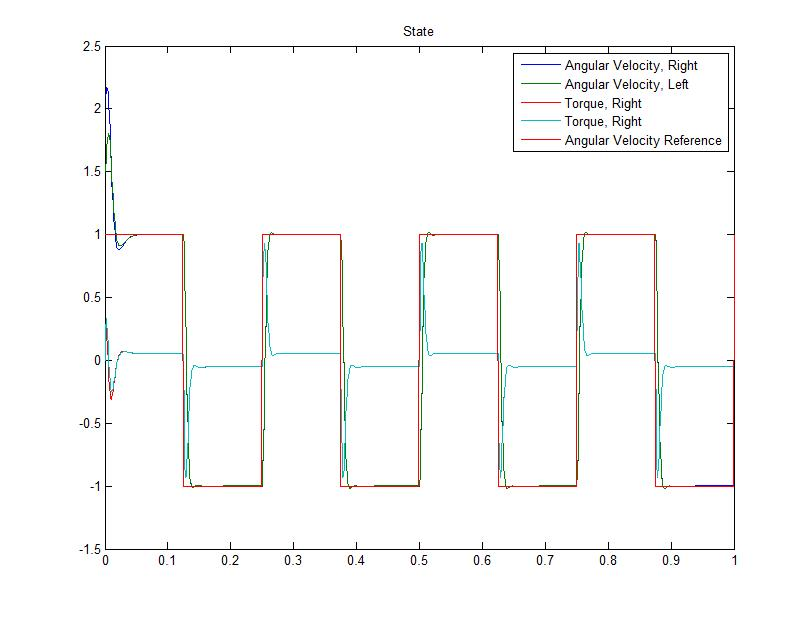
\includegraphics[width=0.75\textwidth]{Certain_State1.jpg}
	\caption{System State with Angular Velocity Reference and Known Parameters}
	\label{fig:ssKpDiagram1}
\end{figure}
\begin{figure}[h]
	\centering
	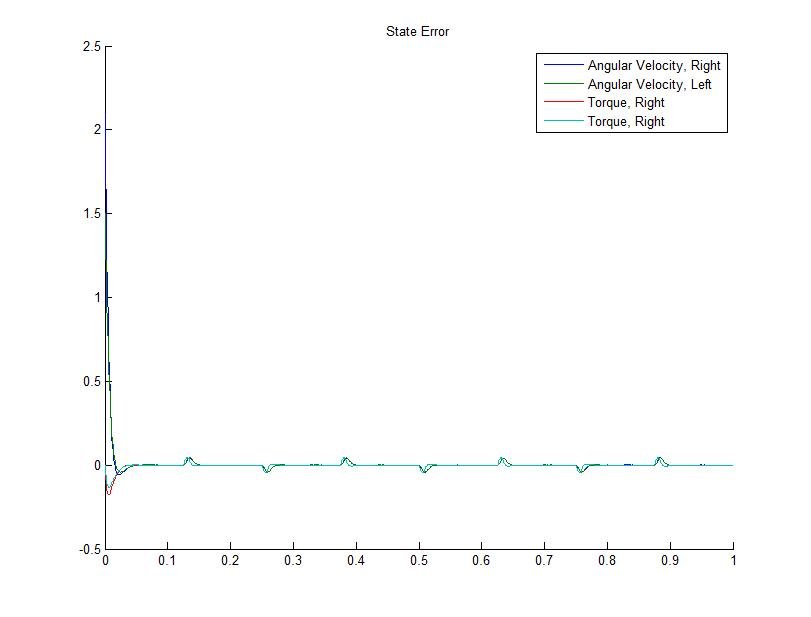
\includegraphics[width=0.75\textwidth]{Certain_StateError1.jpg}
	\caption{State Estimation Error with Known Parameters}
	\label{fig:seKpDiagram1}
\end{figure}

\section{System Performance, Uncertain \mbox{Parameters}}
Without adaptation, the system performance can be seen in figures \ref{fig:ssUpDiagram1} and \ref{fig:seUpDiagram1} when the uncertain parameters are taken to be $k_f = 0.5$, $k_{bwr} = 2\pi$, $k_{bwl} = 2\pi$ in the system model.
\begin{figure}[H!]
	\centering
	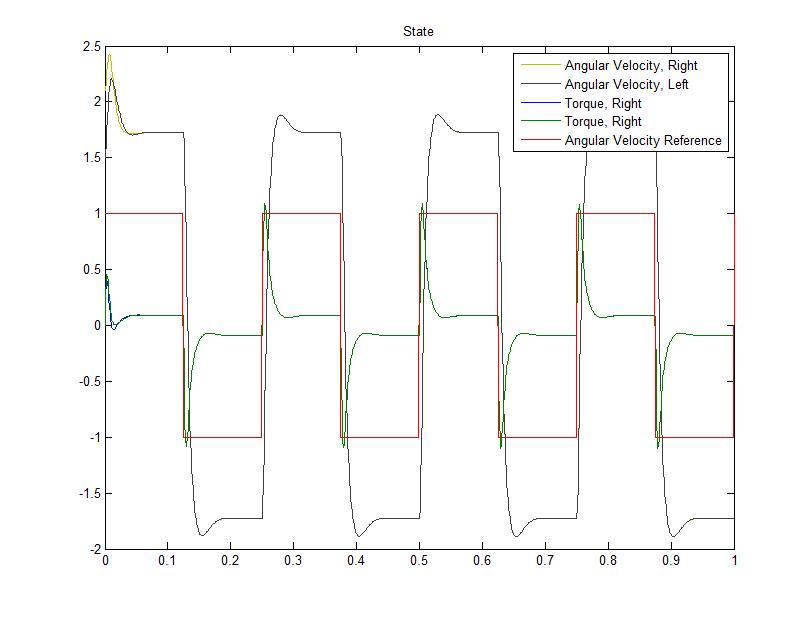
\includegraphics[width=0.75\textwidth]{Uncertain_State1.jpg}
	\caption{System State with Angular Velocity Reference and Uncertain Parameters}
	\label{fig:ssUpDiagram1}
\end{figure}
\begin{figure}[H!]
	\centering
	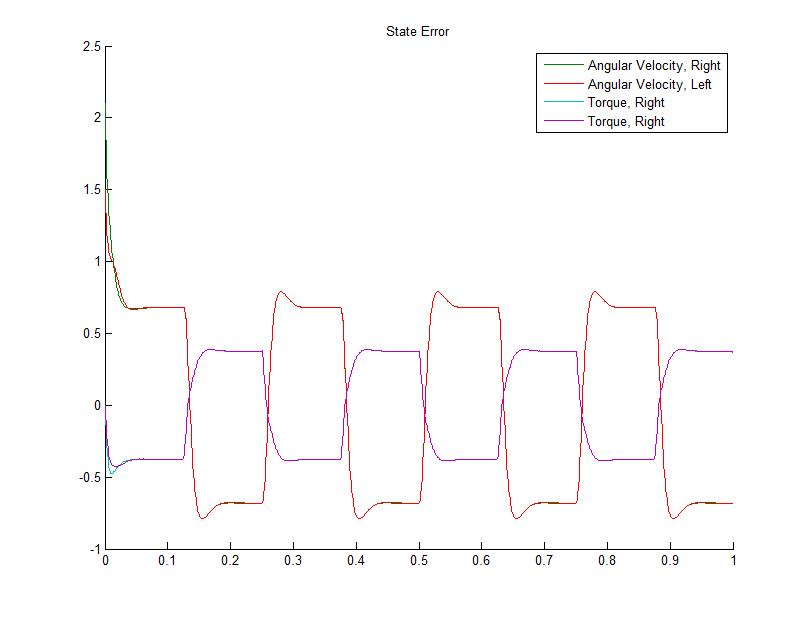
\includegraphics[width=0.75\textwidth]{Uncertain_StateError1.jpg}
	\caption{State Estimation Error with Uncertain Parameters}
	\label{fig:seUpDiagram1}
\end{figure}

\section{System Performance, Adapted \mbox{Parameters}}
With adaptation, the system performance can be seen in figures \ref{fig:ssApDiagram1} and \ref{fig:seApDiagram1} when the uncertain parameters are taken to be $k_f = 0.5$, $k_{bwr} = 2\pi$, $k_{bwl} = 2\pi$ in the system model.
The proportional error coefficients $\gamma_p$ are all taken to be 0.01.
\begin{figure}[H!]
	\centering
	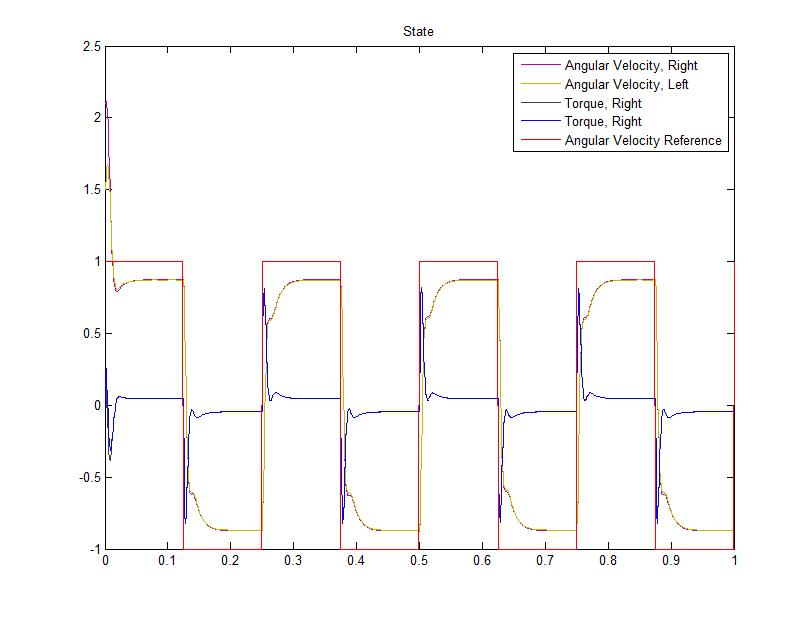
\includegraphics[width=0.75\textwidth]{Adapted_State1.jpg}
	\caption{System State with Angular Velocity Reference and Adapted Parameters}
	\label{fig:ssApDiagram1}
\end{figure}
\begin{figure}[H!]
	\centering
	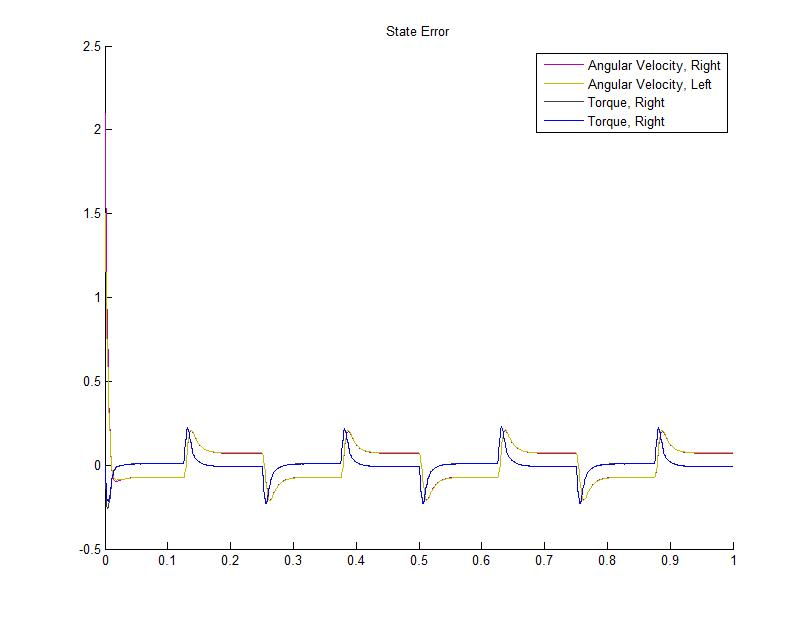
\includegraphics[width=0.75\textwidth]{Adapted_StateError1.jpg}
	\caption{State Estimation Error with Adapted Parameters}
	\label{fig:seApDiagram1}
\end{figure}

\section{System Performance, Time-Varying Parameters}
As a basis for comparison, the performance of the LQG is shown in figures \ref{fig:ssTVpDiagram1} and \ref{fig:seTVpDiagram1} with the time-varying parameters in the system model.
The initial parameters are $k_f = 0.0522$, $k_{bwr} = 20\pi$, $k_{bwl} = 20\pi$.
\begin{figure}[h]
	\centering
	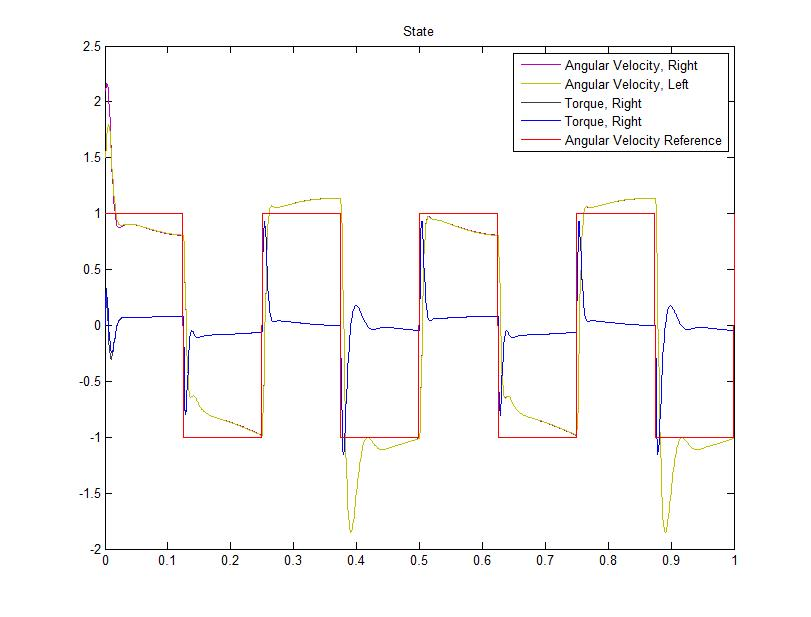
\includegraphics[width=0.75\textwidth]{TV_State1.jpg}
	\caption{System State with Angular Velocity Reference and Time-Varying Parameters}
	\label{fig:ssTVpDiagram1}
\end{figure}
\begin{figure}[h]
	\centering
	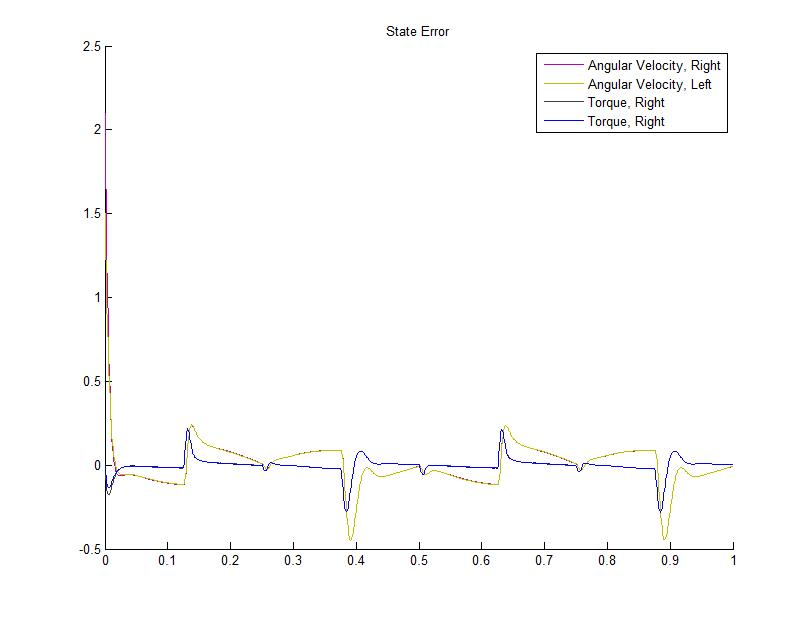
\includegraphics[width=0.75\textwidth]{TV_StateError1.jpg}
	\caption{State Estimation Error with Time-Varying Parameters}
	\label{fig:seTVpDiagram1}
\end{figure}
 
\section{System Performance, Adapted Time-Varying Parameters}
With adaptation, the system performance of the time-varying system can be seen in figures \ref{fig:ssATVpDiagram1} and \ref{fig:seATVpDiagram1} 
when the uncertain parameters are initialized at $k_f = 0.0522$, $k_{bwr} = 20\pi$, $k_{bwl} = 20\pi$ in the system model.
The proportional error coefficients $\gamma_p$ are all taken to be 0.01.
\begin{figure}[h]
	\centering
	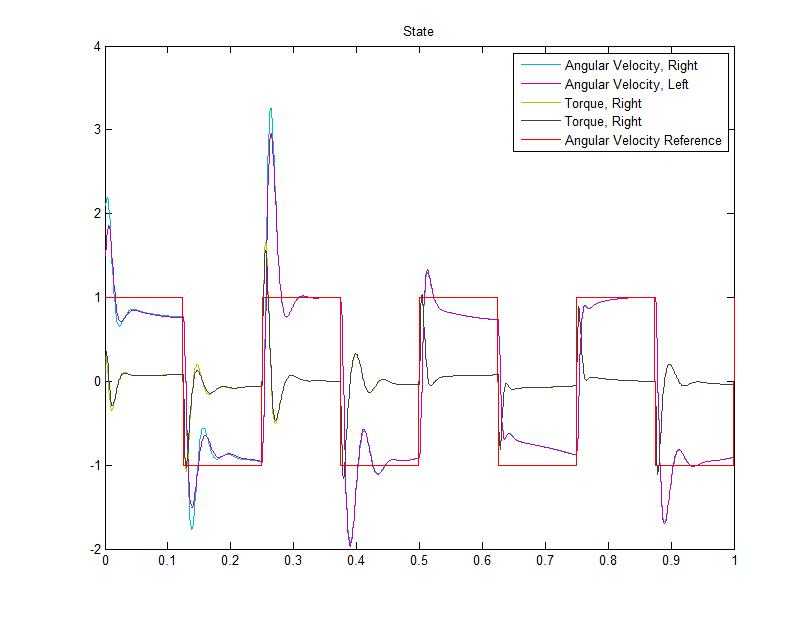
\includegraphics[width=0.75\textwidth]{ATV_State1.jpg}
	\caption{System State with Angular Velocity Reference and Adapted Time-Varying Parameters}
	\label{fig:ssATVpDiagram1}
\end{figure}
\begin{figure}[h]
	\centering
	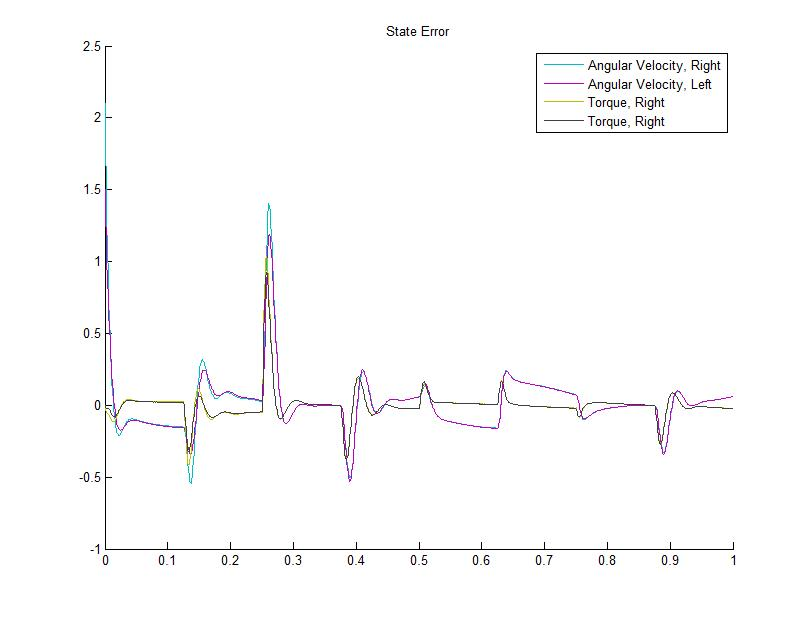
\includegraphics[width=0.75\textwidth]{ATV_StateError1.jpg}
	\caption{State Estimation Error with Adapted Time-Varying Parameters}
	\label{fig:seATVpDiagram1}
\end{figure}


\chapter{Conclusion}
As can be seen by figures \ref{fig:ssUpDiagram1} and \ref{fig:ssApDiagram1}, the performance of the adapted system has reduced the overshoot by half, 
but has developed a steady-state error. An integration term in the adaptation mechanism would most likely correct this problem.
While the adaptation mechanism has improved the performance of the constant parameter uncertainty, as shown in figures \ref{fig:ssTVpDiagram1} and
\ref{fig:ssATVpDiagram1} the adaptation has degraded the performance of the time-varying system. This is likely due to the order of the adaptation not being
able to track a sinusoid.

The results show that the adaptation mechanism improves system performance in the face of uncertain parameters, and could be improved further in order
to track uncertainties. It is likely that this system could track low-frequency step changes in the uncertain parameters with steady-state error. 
Future work will refine the adapter in order to be more robust.


\begin{thebibliography}{9}

\bibitem{ivanjko2010}
  Ivanjko E., Petrinic T., \& Petrinic I.,
  (2010)
  \emph{Modelling of Mobile Robot Dynamics}.
  Paper presented at the 7th EUROSIM Congrees on Modelling and Simulation. 

\end{thebibliography}

\end{document}



